\documentclass{TemplateLecture}

\renewcommand{\LectureName}{Lineare Algebra II}
\renewcommand{\ProfName}{Stefan Schwede}
\renewcommand{\Semester}{SoSe 2024}
\renewcommand{\mName}{Jan Malmström}

\begin{document}

\pagenumbering{arabic}
\section{CW-Complexes}

The name abbreviates compact-Closure-Weak-Topology. They are \enquote{nice} classes of spaces for the purpose of homotopy theory/algebraic topology. They are build by successively attaching cells.

The \(n\)-cell is \(D^n = \set{x \in \IR^n: \abs{x} \leq 1}\). It may also be called \(n\)-balls or \(n\)-discs.
\(S^{n-1} = \partial D^n = \set{x\in \IR^n : \abs{x} = 1}\) is the \(n-1\)-Sphere.
See figure \ref{fig:exDn} for examples.

\begin{figure}
    \centering
    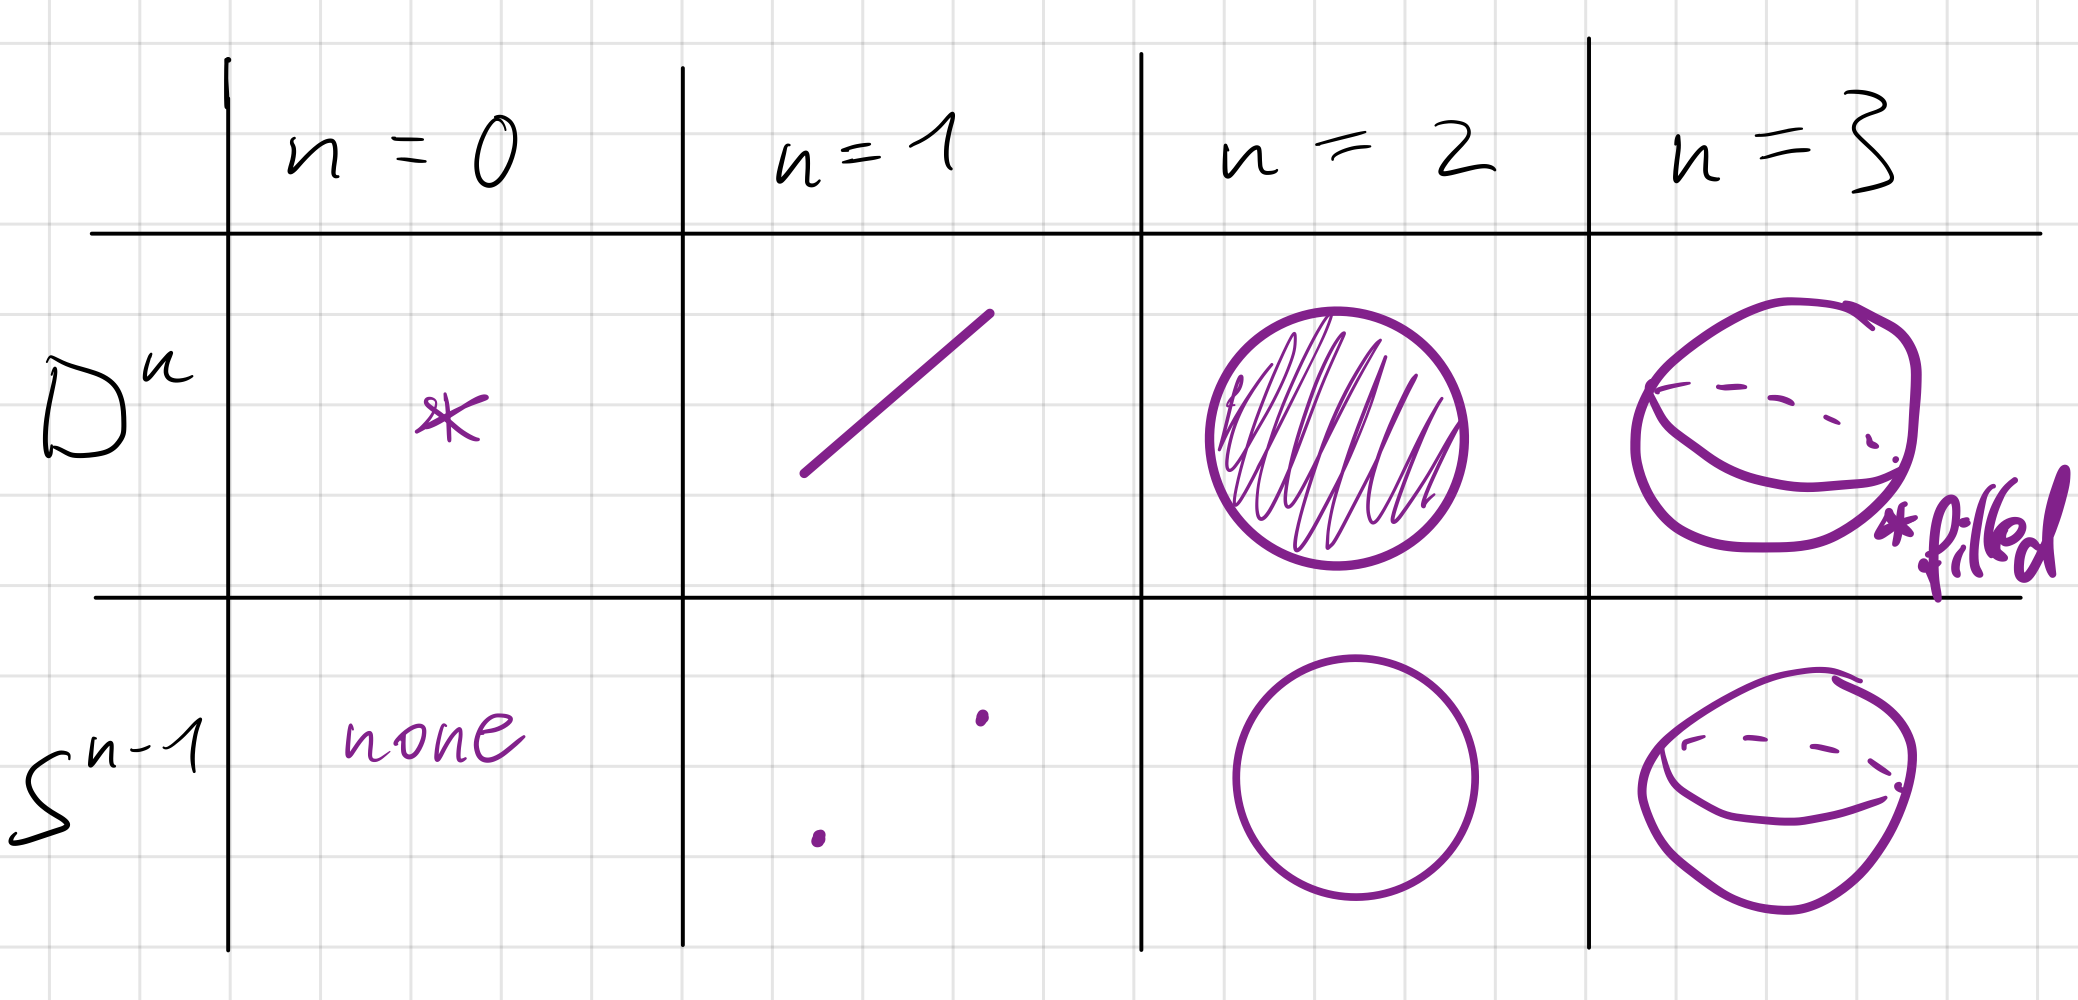
\includegraphics[width=0.8\linewidth]{pic/exDn.png}
    \caption{\(D^n\) and \(S^{n-1}\) for small \(n\)}
    \label{fig:exDn}
\end{figure}


\subsection{Definition}

\begin{construction}
    Let \(n \geq 0\), let \(f\colon S^{n-1} \to X\) be a continuous map, the \emph{attaching map}\index{Attaching map}. We form the quotient space
    \[X \cup_{f, \partial D^n} D^n = X \cup_f D^n = X \cup_{\partial D^n} D^n \coloneq X \amalg D^n/\sim\]
    where \(\sim\) is the equivalencce relation on \(X\amalg D^n\) genearted by \(\forall \; x \in S^{n-1}: f(x) \sim x\).
\end{construction}

\textbf{Terminology.} We say: \enquote{\(X\cup_f D^n\) is obtained by attaching an \(n\)-cell to \(X\) along \(f\)}.

\begin{bsp}
    \begin{itemize}
        \item \(X\cup_f D^0 = X \amalg D^0\)
        \item \(\set{*} \cup_{S^{n-1}} D^n = D^n/ \sim = D^n/ S^{n-1} \cong S^n\)
        
        In this example \(\sim\) identifies all of \(S^{n-1}\) to a point, which then is homeomorphic to \(S^n\)\footnote{supposed as known}.
        
        \item Remark, that the attaching map matters greatly. See figure \ref{fig:exAt}
        \[S^{n-1} \cup_f D^n \cong D^n \quad \text{with } f = \Id\colon S^{n-1} \to S^{n-1}\]
        \[S^{n-1} \cup_f D^n \quad \text{with } f \colon S^{n-1} \to S^{n-1} \text{ constant}\]
        \begin{figure}
            \centering
            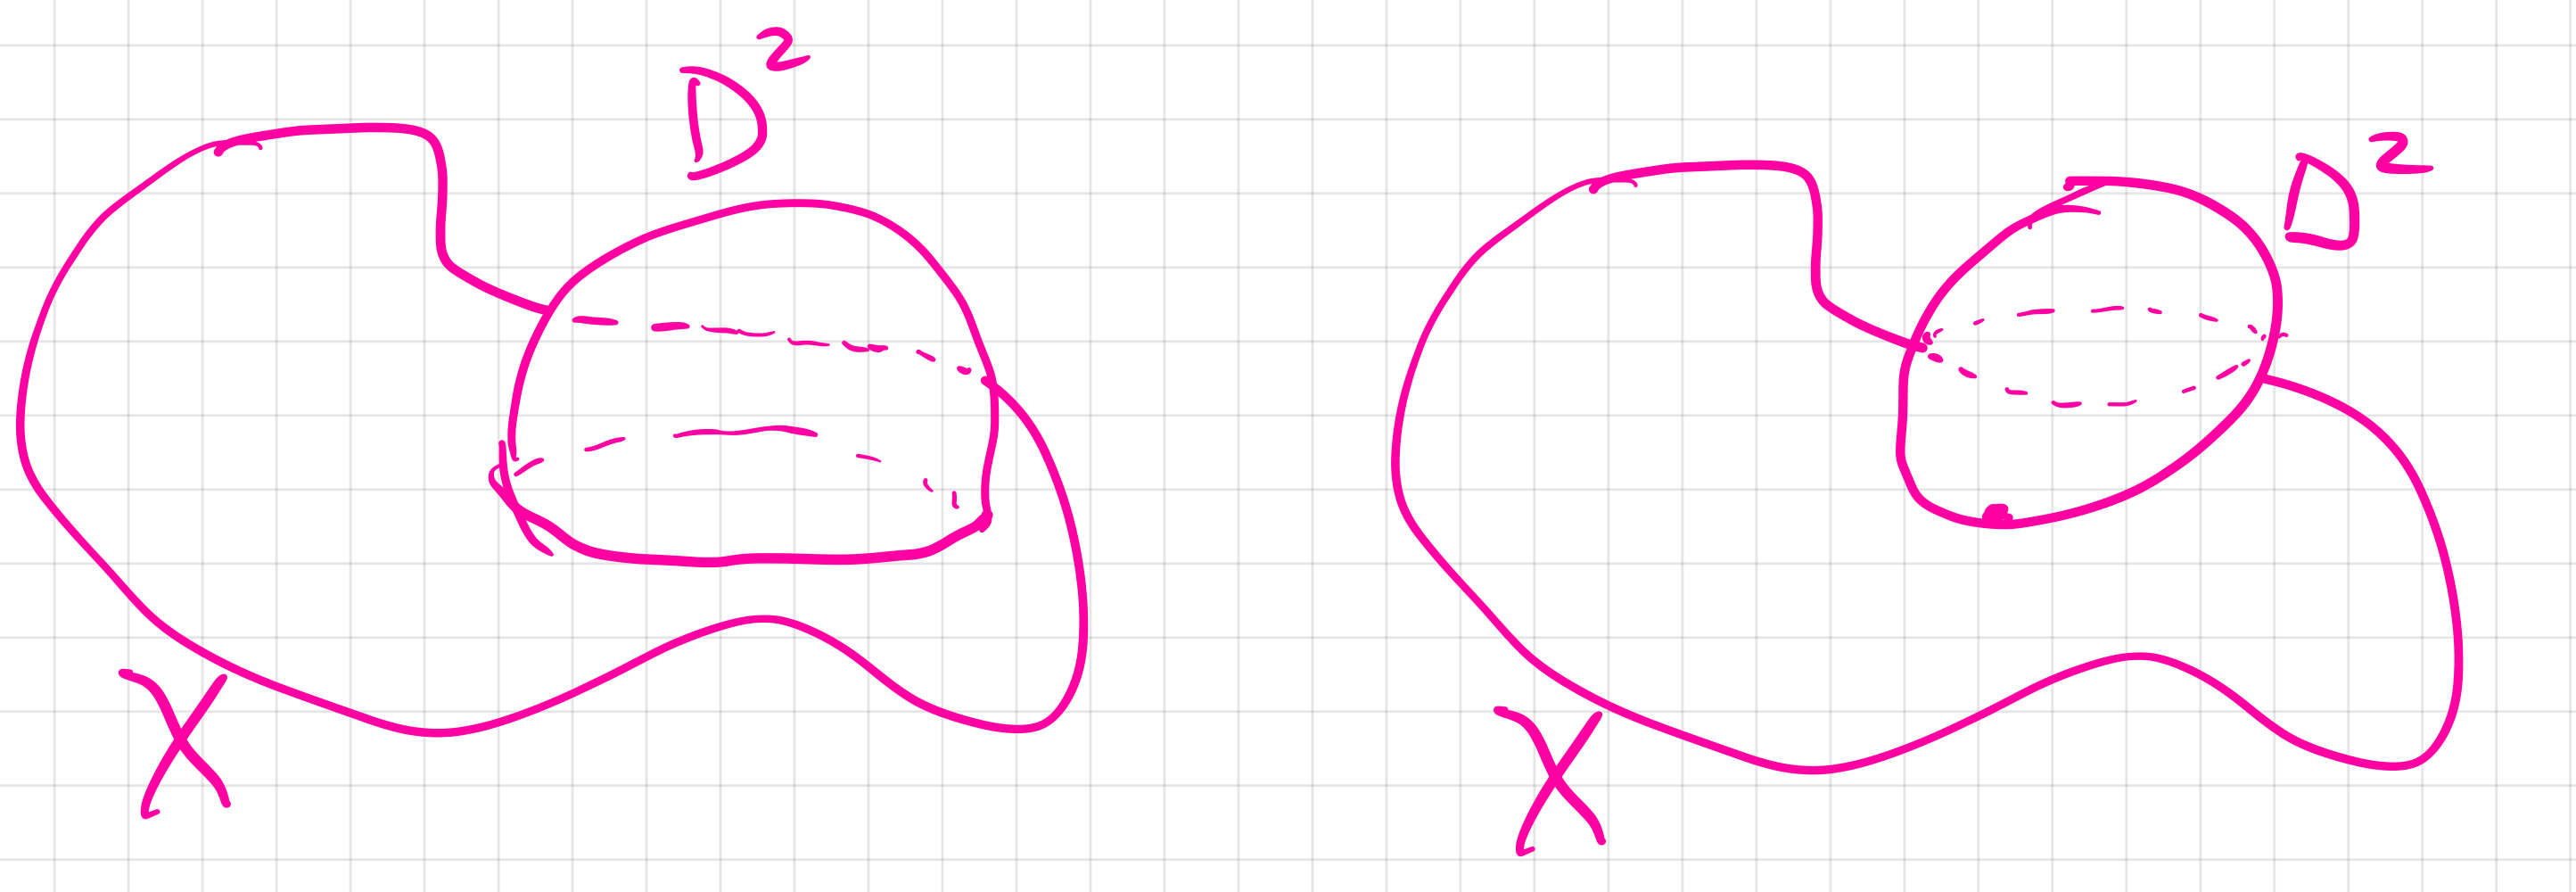
\includegraphics[width=0.8\linewidth]{pic/exAt.png}
            \caption{The attaching map influences how \(D^n\) is attached.}
            \label{fig:exAt}
        \end{figure}
    \end{itemize}
\end{bsp}

\subsubsection*{Simultaneous attachment of several cells}

Let \(J\) be an indexing\footnote{\enquote{indexing}does not carry mathematical meaning} set, considered as a discrete space (\(J = \emptyset\) is allowed).

Give \(J \times D^n\) the product topology, then
\[J \times D^n \cong \coprod_{j \in J} \set{j} \times D^n\text{\footnote{supposed as known}}\]
as a topological space. The \(\coprod\) represents the disjoint union topology.

It follows, that
\[\begin{tikzcd}
    \set{\text{continuous maps } f\colon J \times D^n \to X} \ar[d, phantom, "\cong", sloped] & f \ar[d, mapsto] \\
    \set{\text{J-indexed families of continuous maps } \set{f_j \colon D^n \to X}_{j \in J}} & f_j = f(j, \_)
\end{tikzcd}\]
We will identify them from now on.

\begin{defi}{}{}
    Let \(f \colon J\times \partial D^n \to X\) be a continuous map, the \emph{attaching map}\index{Attaching map}.
    \[X\cup_{f, J\times \partial D^n} J\times D^n = X \cup_f J\times D^n = X \cup_{J\times \partial D^n} J \times D^n \coloneq X \amalg J\times D^n /\sim\]
    where \(\sim\) is the equivalence relation generated by \(f(x) \sim x\) for all \(x \in J\times \partial D^n\).
\end{defi}



\textbf{Remark.} Write
\[p\colon X \amalg J\times D^n \to X\cup_f J\times D^n\]
for the quotient map. From the universal property of the qoutient map follows: Given maps \(g \colon X \to Y\) and \(\Psi_j \colon D^n \to Y\) such that \(g(f_j(x)) = \psi_j(x)\) for all \(j \in J, x \in \partial D^n\) there is a unique map \(\psi\colon X\cup_f J\times D^n \to Y\), such that
\[\psi \circ p = g + \coprod_{j \in J} \psi_j \colon X \amalg (J\times D^n) \to Y\]
and \(\psi\) is continuous iff \(g\) and all \(f_j\) are continuous.

Remeber the quotient-topology: A subset \(O\) in \(X \cup_f J\times D^n\) is open iff \(p^{-1}(O)\) is open in \(X \amalg J\times D^n\). This is equivalent to \(p^{-1}(O) \cap X\) is open in \(X\) and for all \(j \in J\) \(p^{-1}(O) \cap j \times D^n\) is open in \(D^n\).


\(X\) is a closed subspace of \(X\cup_f J\times D^n\) \(J \times \mathring{D^n}\) is an open subset of \(X\cup_f J\times D^n\)
\(X \cup_f J\times D^n\) is as a set (not as a space) the disjoint union of \(X\) and \(J\times \mathring{D^n}\).
We elaborate

\begin{proposition}
    \begin{enumerate}
        \item The composition
        \[\begin{tikzcd}
            X \ar[r] & X\amalg (J\times D^n) \ar[r, "p"] & X\cup_f J\times D^n
        \end{tikzcd}\]
        is a closed embedding (i.e. a closed injective map).
        \item The composition 
        \[\begin{tikzcd}
            J\times \mathring{D^n} \ar[r, hook, "incl"] & J\times D^n \ar[r] & X\amalg J\times D^n \ar[r, "p"] & X \cup_f J \times D^n
        \end{tikzcd}\]
        is an open embedding (i.e. injective and open)
        \item The underlying set of \(X\cup_f J\times D^n\) is the disjoint union of the image of \(X\) and \(J\times \mathring{D^n}\).
    \end{enumerate}
\end{proposition}

\begin{proof}
    Suppose \(M \subseteq X \amalg J\times D^n\) is saturated, i.e. \(M = p^{-1}(p(M))\). If \(M\) is saturated and open, then \(p(M)\) is open in \(X\cup_f J\times D^n\).
    \begin{enumerate}
        \item \begin{description}
            \item[\(n = 0\)] \(X\cup J\times D^0 = X \amalg J\times D^0\) is obvious.
            \item[\(n \geq 1\)] let \(r\colon D^n \to S^{n-1}\) be a map, such that \(r(x) = x\) for all \(x \in S^{n-1}\).This \underline{cannot} be done continuously.
            Define \(X \amalg J\times D^n \to X\) by \(x \mapsto x, (j,y) \mapsto r(y)\). This is compatible with the equivalence relation, so it descends to a (noncontinuous) map \(X \cup_f J\times D^n \to X\). This prooves injectivity.
            To show this is a closed map, we consider a closed subset \(A \subseteq X\). Then
            \(p^{-1}(p(A)) = A\amalg f^{-1}(A) \subseteq X\amalg J\times D^n\)
            \(\subset J\times \partial D^n \subset J\times D^n\) is closed in \(X \amalg J\times D^n\).
            So \(p(A)\) is closed in \(X\cup_f J\times D^n\).
        \end{description}
        \item All points in \(J \times \mathring{D^n}\) are their own equivalence classes, so the map is injective. To show that the map of 2. is open, we let \(B\) be an open subset of \(J\times \mathring{D^n}\). This is then also open in \(J \times D^n\). \(p^{-1}(p(B)) = \emptyset \amalg B\subset X\amalg J\times D^n\) open, so \(p(B)\) is open in \(X\cup_f J\times D^n\).
        
        \item I think this was prooven with a picture I didn't draw.
    \end{enumerate}
\end{proof}

\textbf{Exercise.} Let \(V_j\) be an open subset of \(D^n\) for every \(j \in J\), such that \(V_j \supset \partial D^n\). Show, that the set \(V = X \cup \bigcup_{j \in J} V_j\) is open in \(X\cup_f J\times D^n\).

From now on we often identify \(X\) with its image in \(X \cup_f J\times D^n\) and \(J\times \mathring{D^n}\) with its image in \(X \cup_f J\times D^n\)

\begin{defi}{Compactness}{}
    A space \(X\) is \emph{compact}, if it is Hausdorff (any two points can be separated by two disjoint open sets) and \emph{quasicompact} (any open cover has a finite subcover).
\end{defi}

\textbf{Remark.} Some literature defines compactness equivalent to quasicompactness. This lecture uses the definition that was given.

\begin{thm}{}{comp}
    Let \(f\colon J \times \partial D^n \to X\) be a continuous attaching map.
    \begin{itemize}
        \item If \(X\) is Hausdorff, then so is \(X \cup_f J\times D^n\).
        \item If \(X\) is compact and \(J\) is finite, then \(X \cup_f J\times D^n\) is compact.
        \item Let \(K\) be a quasicompact subset of \(X\cup_f J\times D^n.\) Then \(K\cap (\set{j} \times \mathring{D^n}) = \emptyset\) for almost all\footnote{mathematical term for all but finitely many.} \(j \in J\).
    \end{itemize}
\end{thm}

\begin{lem}{}{}
    There exists an open neighborhood \(V\) of \(X\) in \(X\cup_f J\times D^n\) and a continuous map \(r\colon V\to X\) that is the identity on \(X\). (\(X\) is a neighborhood retract inside \(X \cup_f J\times D^n\)).
\end{lem}

\begin{proof}
    \begin{figure}
        \centering
        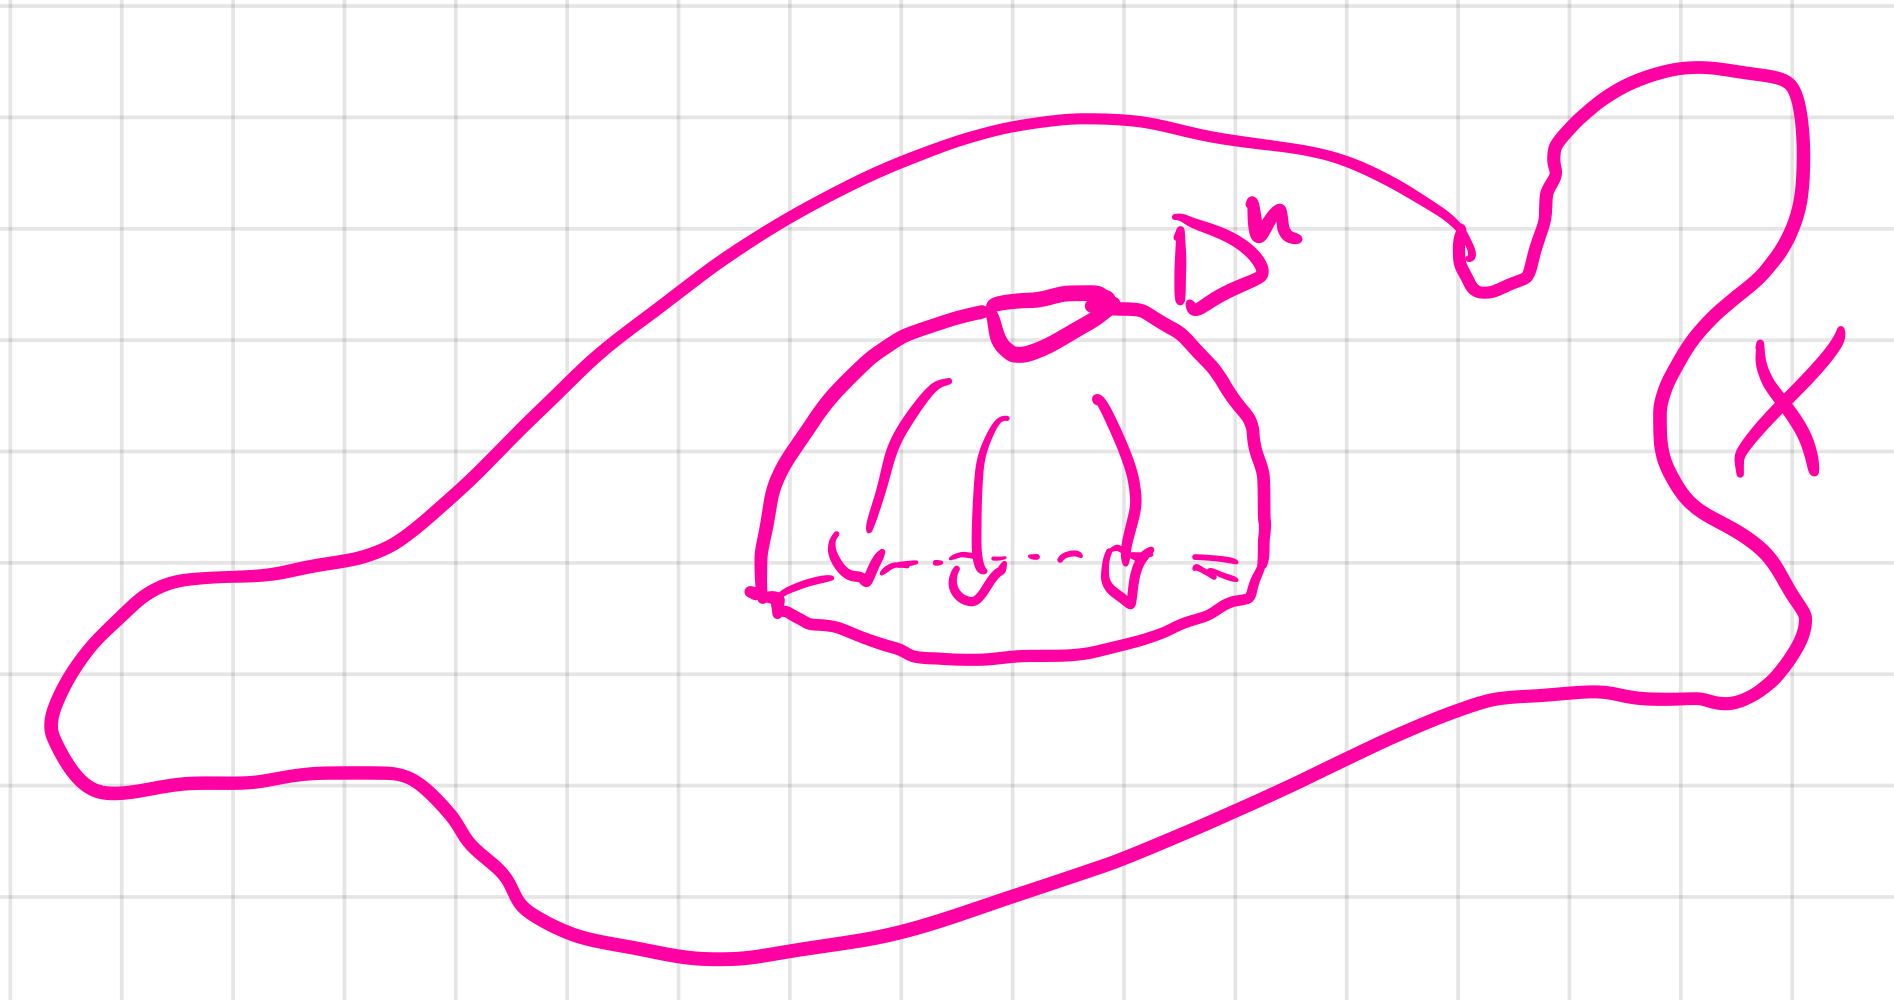
\includegraphics[width=0.8\linewidth]{pic/exRt.png}
        \caption{If a point in \(D^n\) is missing, it can be continuously retracted.}
        \label{fig:exRt}
    \end{figure}
    See figure \ref{fig:exRt}. We take
    \(V = X\cup_{J\times \partial D^n} J\times (D^n\setminus {0})\). This is open in \(X \cup_f J\times D^n\). We define \(r \colon V\to X\) by \(x\mapsto x, (j,z) \mapsto f(j, z/\abs{z})\).
\end{proof}

\begin{proof}[Proof of theorem \ref{thm:comp}]\leavevmode
    \begin{enumerate}
        \item \begin{description}
            \item[Case 1] \(x,y \in J\times \mathring{D^n}\). Since \(\mathring{D^n}\) is Hausdorff, so is \(J\times \mathring{D^n}\), so we can separate \(x\) and \(y\) by open disjoint subsets in \(J\times \mathring{D^n}\), Since \(J\times \mathring{D^n}\) is open in \(X \cup_f J\times D^n\), theses subsets are also open in \(X\cup_f J\times D^n\).
            \item[Case 2] \(x\in X, y \in \set{j} \times \mathring{D^n}\). We choose an \(y \in O_y \subset j \times D^n\) open \(j \times \partial D^n \subseteq V_j \subseteq j\times D^n\) s.t. \(O_j \cap V_j = \emptyset\).
            Then \(V\coloneq X\cup V_j \cup \bigcup_{k \in J\setminus\set{j}} D^n\) is open\footnote{by an exercise.} in \(X \cup_f J \times D^n\). \(V \cap O_j = \emptyset\), \(x \in V, y \in O_j\).
            \item[Case 3] \(x,y \in X\). Since \(X\) is Hausdorff, there are open subsets \(O_x, O_y\) of \(X\) with \(x \in O_x\), \(y \in O_y\), \(O_x \cap O_y = \emptyset\).
            We let \(V\) be an open subset of \(X \cup_f J \times D^n\) with a continuous retraction \(r\colon V\to X\), \(r\rvert_X = \Id_X\). Then \(x \in r^{-1}(O_x), y \in r^{-1}(O_y)\), \(r^{-1}(O_y), r^{-1}(O_y)\) are open, and disjoint.
        \end{description}
        \item If \(X\) is compact and \(J\) is finite, then \(X\amalg J\times D^n = X \amalg \coprod_{j \in J} \set{j} \times D^n\) is compact hence also the quotient space \(X \cup_f J\times D^n\) is quasi-compact. Hausdorff is inherited by \(1.\).
        \item Let \(K\) be a quasicompact subset of \(X \cup_{J\times \inner{D^n}} J\times D^n\). We define subsets \(V_j\) of \(D^n\) for all \(j \in J\) as follows: If \(K \cap (j \times \mathring{D^n}) = \emptyset\), we set \(V_j = D^n\). If \(K \cap (j\times \mathring{D^n}) \neq \emptyset\), we choose a \(V_j\), that doen't contain at least one point of \(K\), is open, and contains \(\partial D^n\). Now
        \[(X\bigcup_{j \in J} V_j) \cup \bigcup_{j \in J} \set{j} \times \mathring{D^n}\]
        is an open cover of \(X\cup_f J\times D^n\). Since \(K\) is quasicompact, there is a finite subset \(L\) of \(J\) such that
        \[K \subset (X\cup_{j \in J} V_j) \cup \bigcup_{j \in L} \set{j} \times \mathring{D^n}.\]
    \end{enumerate}
\end{proof}

\begin{bsp}[Hawaiian Earrings]
    The set
    \[H = H_1 \cup H_2 \cup H_3 \cup \dots = \bigcup_{i \geq 1} H_i\]
    wherein \(H_i\) is the circle in \(\IR^2\) with radius \(1/i\) and center \((1/i, 0)\), equipped with the subspace topology of \(\IR^2\) is called the Hawaiin earrings (see figure \ref{fig:exHw}).
    \begin{figure}
        \centering
        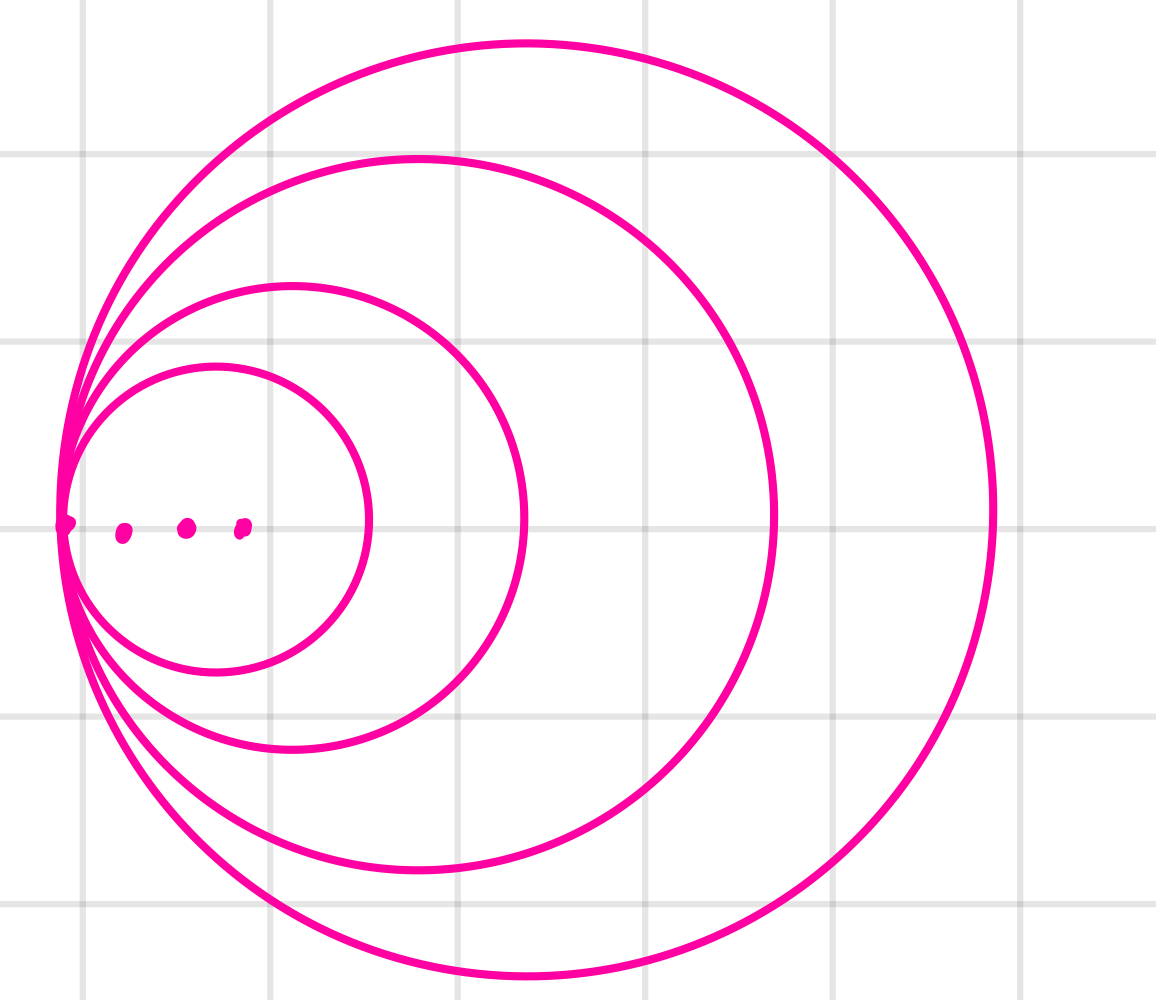
\includegraphics[width=0.5\linewidth]{pic/exHw.png}
        \caption{Hawaiian earrings}
        \label{fig:exHw}
    \end{figure}

    Is \(H\) obtained from \(\set{(0,0)}\) by attaching countably many 1-cells? It is not.

    Consider a continuous map \(\psi_j\colon D^l = [-1,1]\) such that it is a surjective, and \([-1,1]/-1\sim 1\) onto  \(H_j \subset H\) is a homeomorphism.

    \[\set{(0,0)} \amalg \IN \times D^1 \to H, \quad (j,x) \mapsto \psi_j(x)\]
    is a continuous surjection. Then
    \[\set{(0,0)} \cup_{\IN\times \partial D^1} \IN \times D^1 \to H\]
    is a continuous bijection. However, it is not a homeomorphism.

    Consider \(V = \set{(0,0)} \cup_{\IN \times \partial D^1} \IN \times ([-1,0) \cup (0,1])\). This is open in \(\set{(0,0)} \cup_{\IN\times \partial D^1} \IN \times D^1\). Its complement is closed, but the image of that complement, \((1/n,0)_{n\in \IN}\) is not closed in \(H\).
\end{bsp}

\begin{defi}{CW-Complex}{cwcomplex}
    A relative \emph{CW-complex}\index{CW-} is a space \(X\) equipped with a sequence of closed subspaces
    \[A = X_{-1} \subseteq X_0 \subseteq X_1 \subseteq \dots \subseteq X_n \subseteq \dots \]
    such that
    \begin{enumerate}
        \item For every \(n \geq 0\) \(X_n\) can be obtained from \(X_{n-1}\) by attaching \(n\)-cells.
        \item \(X = \bigcup_{n \geq 0} X_n\) and \(X\) has the weak topology with respect to the sequences.
    \end{enumerate}

    precisely:
    \begin{enumerate}
        \item There exists an index set \(J\), a continuous map \(f \colon J \times \partial D^n \to X_{n-1}\) and a homeomorphism \(\psi\colon X_{n-1} \cup_f J\times D^n \to X_n\) that is the identity on \(X_{n-1}\).
        \item A subset \(O\) of \(X\) is open in \(X\) iff \(O\cap X_n\) is open in \(X_n\) for all \(n \geq 0\).
    \end{enumerate}
\end{defi}

    \textbf{Remark.} 2. is equivalent to: A subset \(C\) of \(X\) is closed in \(X\) iff \(C\cap X_n\) is closed in \(X_n\) for all \(n \geq 0\).

    2. implies, that a map \(f\colon X\to Y\) is already continuous if \(f\rvert_{X_n}\colon X_n \to Y\) is continuous for all \(n \geq 0\).

\begin{notation}
    We usually say \((X,A)\) is a relative \(CW-complex\) and leave the \(X_n\) implicit.

    For \(A = \emptyset\) \(X\) is called a absolute CW-complex, or just a CW-complex.

    The subspace \(X_n\) in a CW-complex is the \(n\)-skeleton.

    A relative CW-complex \((X,A)\) is finite-dimensional if \(X_n = X\) for some \(n \geq 0\).

    A relative CW-complex \((X,A)\) is finite, if there are only finitely many cells altogether.

    Once chosen a homeomorphism \(\psi\) as above, then the characteristic map  of the \(j\)-th \(n\)-cell is the composite
    \[\begin{tikzcd}
        D^n \ar[r, "{(j, \_)}"] & X_{n-1}\cup_{J\times \partial D^n} J \times D^n \ar[r, "\psi", "\cong"'] & X_n \ar[r, hook] & X
    \end{tikzcd}\]

    \(X_j\rvert_{\mathring{D^n}} \mapsto X_j(\mathring{D^n})\) is a homeomorphism  ... , which is one path component of \(X_n \setminus X_{n-1}\). The restriction \(f_j \colon X_j\rvert_{\partial D^n} \to X_{n-1}\) is called the attaching map as before.
\end{notation}

Comment: The space \(X_n \setminus X_{n-1}\) is a disjoint union of open cells \(\mathring{D^n}\). So the indexing set could be taken as \(\pi_0(X_n\setminus X_{n-1})\).

For every path-component of \(X_n \setminus X_{n-1}\) there exists a homeomorphism \(f \colon \mathring{D^n} \to pathcomponent\), that extends to a continuous map \(\bar f \colon D^n \to X_n\).


\begin{example}
    Any discrete space is an absolute \(0\)-dimensional CW-complex.

    Let \(z \in S^n\) be any point. Then  the minimal CW-structure on \(S^n\) is \(X_{-1} = \emptyset, X_0 = \set{z} = X_1 = \dots = X_{n-1}\) \(X_n = X_{n+1} = \dots = S^n\). It consists of 1 \(0\)-cell and 1 \(n\)-cell. 

    \(S^n \cong D^n / \partial D^{n-1}\) \(z \leftarrow \partial D^{n-1}\)

    Example \(X = S^n\) \(n \geq 2\) Another CW-structure:

    picture

    \(X_{-1} = \emptyset, X_0 = X_1 = \dots = X_{n-2} = \set{(1,0,\dots, 0)}\) \(X_{n-1} = equator = \set{(x,0) : x \in S^{n-1}}\)
    \(X_n = X_{n+1} = \dots = S^n\)
    1 0 cell 1  \(n-1\)-cell 2 \(n\)-cells
    \(S^n \cong D^n \cup_{S^{n-1}} D^n\)

    Example: \(S^2\) 2 1 cell 2 2 cell 2 0 cell 
    picture

    Analog for \(S^n\) is a CW-complex with \(2\) \(i\)-cells for \(i = 0, \dots, n\).

    On \(S^1\) pick any finite subset \(A \subseteq S^1\). Then \(S^1\) has a CW-structure with \(X_{-1} = \emptyset, X_1 = A, X_2 = S^1\). n 0 cells n 1 cells.

    Any non-discrete space, that admits an absolute CW-structure admits uncountably many different CW-structures.

    Preview: The Euler characteristic of a finite absolute CW-comples is \(\chi(X) = \sum_{n \geq 0} (-1)^n \#n\text{-cells}\) does not depend on the CW-structure. We will eventually show this using singular homology. 
\end{example}

Then: Let \((X,A)\) be a relative CW-complex.
\begin{enumerate}
    \item If \(A\) is Hausdorff, then so is \(X\).
    \item If \(A\) is compact and \((X,A)\) is finite, then \(X\) is also compact.
\end{enumerate}

\begin{proof}
    Because \(X_{-1} = A\) is Hausdorff and \(X_n\) can be obtained from \(X_{n-1}\), by attaching cells, inductively \(X_n\) is Hausdorff for all \(n \geq 0\).
    Claim: Let \(O_n, P_n\) be open disjoint subsets of \(X_n\). Then there exist disjoint open subsets \(O_{n+1}, P_{n+1}\) of \(X_{n+1}\), such that \(O_n = O_{n+1} \cap X_n, P_n = P_{n+1} \cap X_n\).
    \begin{proof}
        Since \(X_{n+1}\) can be obtained from \(X_n\) by attaching \((n+1)\)-cells \(X_n\) is a neighborhood retract in \(X_{n+1}\), i.e. there are open neighborhood \(V\) of \(X_n\) in \(X_{n+1}\) and a continuous retraction \(r\colon V\to X_n\) with \(r \rvert_{X_n} = \Id\). We set \(O_{n+1} = r^{-1}(O_n), P_{n+1} = r^{-1}(P_n)\).

        Proof of the Hausdorff property: Let \(x,y \in X\) be disjoint points. Since \(X = \bigcup_{n \in \IN} X_n\). then for some \(n \geq 0\), \(x,y \in X_n\). Since \(X_n\) is Hausdorff, there are open, disjoint subsets \(O_n, P_n\) of \(X_n\) with \(x \in O_n, y \in P_n\). Inductiveleuse the claim to find open disjoint subsets \(O_m\), \(P_m\) of \(X_m\) for all \(m \geq n\), such that \(O_{m+1} \cap X_m = O_m, P_{m+1} \cap X_m = O_m\) for all \(m \geq n\). Then set \(O = \bigcup_{m \geq n} O_m, P = \bigcup_{m\geq n} PM\) disjoint subsets of \(X\) and open in \(X\) by the weak topology, as \(O\cap X_m = O_m\) open in \(X_m\).
    \end{proof} 

    Induction of \(n\) such that \(X_n\) is compact because \(X_n\) is obtained from \(X_{n-1}\) by attaching finitely many cells. Also \(X = X_n\)for sufficently large \(n\). So \(X\) is compact.
\end{proof}

Note: Suppose that \(X\) admits a CW-structure. Then the following are equivalent: \(X\) admits a finite CW-structure \(\Lra\) \(X\) is compact.

From now on standing assumption: the base \(A\) in a relative CW-complex \(X,A\) is Hausdorff.Then \(X\) is also Hausdorff.

Thus: Let \(X,A\) be a relative CW-complex.

\begin{enumerate}
    \item The closure of every open \(n\)-cell (\(=\) path component of \(X_n\setminus X_{n-1}\)) is compact.
    \item Let \(\chi\colon D^n \to X\) be a characteristic map for some \(n\)-cell, then  the image \(\chi(D^n)\) is the closure of the open cell \(\chi(\mathring{D^n})\)
    \item Let \(U\) be a subset of \(X\) s.t. \(A\subseteq U\). Suppose that the intersection of \(U\) with the closure of every cell is closed. Then \(U\) is closed in \(X\).
\end{enumerate}

Warning: the closure of a cell is not necessary a closed cell:

minimal CW-tructure on \(S^2\) open 2-cell \(S^2\setminus \set{z}\) closure \(= S^2 \neq D^2\).

\begin{proof}
    \begin{enumerate}
        \item By definition every open \(n\)-cells admits a characteristic map \(\chi\colon D^n \to X_n\) continuous s.t. \(\chi\rvert_{\mathring{D^n}}\) is a homeomorphis onto the open cells. Then \(\chi(D^n) \subseteq closure of open cell \chi(\mathring{D^n})\) so they are the same.
        %%hlep

        \item Let \(U\subseteq X\) be as in \(2\). It suffices to show that \(U\cap X_n\) is closed in \(X_n\) for all \(n \geq 0\) (weak topology). We argue by induction on \(n\).
        \(n = -1\) \(U\cap X_{-1} = U\cap A = A\) closed in \(A = X_{-1}\).
        \(n \geq 0\) We choose a homeomorphism \(\psi\colon X_n \cong X_{n-1} \cup_{J\times \partial D^n} J\times D^n\) that is the in?? on \(X_{n-1}\). We let \(p\colon X_{n-1} \amalg J\times D^n \to X_{n-1} \cup_{J\times \partial D^n} J\times D^n \psi \cong \to X_n\) be the ?? 

        \(p^{-1}(U\cap X_n = (U\cap X_{n-1}) \amalg \coprod_{j \in J} p^{-1}(U\cap closure of j-th n-cell))\) closed by hypothesis \(\subseteq X_{n-1} \amalg J\times D^n\)
        \(\implies\) \(U\cap X_n\) is closed in \(X_n\)
    \end{enumerate}
\end{proof}

Rop: Let \(A\) be a Hausdorff-space, \(X = A \cup_f J\times D^n\) obtained from \(A\) by attaching \(n\)-cells. Let \(Y \subseteq X\) be a subspace, such that.
\(Y \cap A\) is closed in \(A\)
\(Y\) can be obtained from \(A \cap Y\) by attaching \(n\)-cells.
\(Y \cap (J\times \inner{D^n})\) is a union of path components of \(J\times \inner{D^n}\).
Then \(Y\) is closed in \(X\).

\begin{proof}
    Claim: If \(Y \cap \set{j} \times \inner{D^n} \neq \emptyset\) (\(\Lra\) \(j\times D^n inner \subseteq Y\)).
    Then \(Y\) contains the closure of \(j\times \inner{D^n}\) in \(X\). ( = the closure of this cell).

    \begin{proof}
        \(Y\) can be obtained from \(Y \cap A\) by attaching \(n\)-cells and \(Y\setminus (Y\cap A)\) is a union fo some of the open cells of \(X\setminus A = J\times \inner{D^n}\). Let \(\chi \colon D^n \to Y\) be a characteristic map for the attaching of the \(j\)-th \(n\)-cell to \(Y\).
        \(\chi(\inner{D^n}) = j \times \inner{D^n}\). Since \(D^n\) is compact, \(f(D^n)\) is quasicompact, and hence closed since \(X\) is Hausdorff. So \(j\times \inner{D^n} = \chi(D^n inner) \subseteq \chi(D^n) \subseteq Y \subseteq X\) closed so the closure of \(\chi\inner{D^n} = j \times \inner D^n\) is in \(\chi(D^n)\) is closed in \(Y\).

        We let \(p\colon A \amalg J\times D^n \to A \cup_f J\times D^n = X\) be the quotient map. Then 
        \(p^{-1}(Y) = (Y\cap A) \amalg \coprod_{j \in J Y \cap (j\times \inner{D^n}) \neq \emptyset} j\times D^n \amalg \coprod_{j \in J Y\cap (j\times \inner D^n) = \emptyset} p^{-1}(Y\cap A) \cap (j\times D^n)\) closed in \(j\times D^n\).
    \end{proof}
    %hlep
\end{proof}

Let \(X,A\) be a relative CW-complex and \(Y\) a closed subspace of \(X\) with \(A \subseteq Y\). Suppose that for all \(n \geq 0\), \(Y \cap X_n \setminus X_{n-1}\) is a disjoint union of path components of \(X_n \setminus X_{n-1}\). Then \(Y, A\) is a relative CW-complex with respect to the induced filtration.
i.e.
\(A = Y_{-1} \subseteq Y_0 = (X_0 \cap A) \subset eq Y_1 = X_1 \cap Y \dots\) %hlep

\begin{proof}
    \begin{enumerate}
        \item \(Y_n\) can be obtained from \(Y_{n-1}\) by attaching \(n\)-cells.
        let \(I = \set{j \in J\colon Y \cap (j\times\inner {D^n}) \neq \emptyset} = \set{j \in J : j\times \inner{D^n} \subseteq Y}\)
        let \(\chi_j \colon D^n \to X_n \subset eq X\) be a charactreistic map for the \(j\)-th \(n\)-cell of \(X\).
        If \(j \in I\), the \(\chi(D^n) = \text{closure of} \chi(\inner{D^n}) in\), hence closed in \(Y\) (\(Y\) closed).
        So we can, and will, consider \(\chi\) as a map with target \(Y\cap X_n = Y_n\).
        We get a continuous map \(\psi \colon Y_{n-1} \cup_{I\times \partial D^n} I\times D^n \to Y_n\) (induced \(\cup \coprod_{j \in J} \chi_j\)),
        which is bijective because source and target are - as sets - both the disjoint union of \(Y_{n-1}\) and \(I \times \inner{D^n}\). We argue, that \(\psi\) is a closed map and hence a homeomorphism.

        \(Y_{n-1} \amalg I\times D^n\) arrow inclusion \(X_{n-1} \amalg J\times D^n\)
        q quotient map          p quotient map.
        \(Y_{n-1} \cup_{I \times \partial D^n} I\times D^n\) arrow \(\psi\) \(Y_n \subseteq X_n\) closed%%tikz

        Let \(B\subseteq Y_{n-1} \cup_{I\times \partial D^n} I\times D^n\) be a closed subset, where \(f_j \colon \partial D^n \to X_{n-1}\) is the attaching map for the \(j\)-th \(n\)-cell i.e. \(f_j = \chi_j\rvert_{\partial D^n}\) Then
        \(p^{-1}(\psi(B)) = q^{-1}(B)_{closed in Y \amalg I\times D^n, hence also in X_{n-1} \amalg J\times D^n} \cup \amalg_{j \in J\setminus I} j\times f_j^{-1}(B \cap X_{n-1})\) \(J\setminus I) \times D^n\) closed in \(J\setminus I) \times D^n\).

        \item \(Y\) has the weak topology with respect  \(Y = Y \cap X = Y \cap (\bigcup_{n \geq 0} X_n) = \bigcup_{n \geq 0} (Y \cap X_n) = \bigcup_{n \geq 0} Y_n\).
        let \(B \subseteq Y\) be a subset such that for all \(n \geq 0\), \(B\cap Y_n\) is closed in \(Y_n\). Since \(Y\) is closed in \(X\), \(Y_n\) is closed in \(X_n\), so \(B\cap Y_n is closed in X_n\). Since \(X\) has the weak topology, \(B\) is closed in \(X\), hence also in \(Y\).
    \end{enumerate}
\end{proof}

\begin{defi}{}{}
    A CW-subcomplex of a relative CW-complex \((X,A)\) is a closed subspace \(Y\) of \(X\), such that \(A \subseteq Y\) and for all \(n \geq 0\) \(Y \cap (X_n\setminus{X_{n-1}})\) is a union of path components of \(X_n\setminus X_{n-1}\)
\end{defi}

Then \((Y,A)\) is a relative CW-complex with respect to the induced filtration.

\begin{thm}{}{}
    Let \((X,A)\) be a relative CW-complex.
    \begin{enumerate}
        \item The closure of every cell is contained in a finite subcomplex.
        \item Every compact subset of \(X\) is contained in a finite subcomplex of \(X\).
    \end{enumerate}
\end{thm}

Remark Historically first definition of CW-complex (J.H.C. Whitehead): A CW-complex is a space X equipped with a decomposition \(X = \dot\bigcup_{n \geq 0, i \in J_n} e_i^n\), such that
\begin{enumerate}
    \item \(e_i^n\) is homeomorphic do \(\inner{D^n}\).
    \item The closure of \(e_i^n\) is contained in the union of finitely many \(e^m_j\)-s (\enquote{closure finite}).
    \item a subset \(Y\) of \(X\) is closed iff \(Y \cap \overline{e_i^n}\) is closed for all \(e_i^n\). then called weak topology.
\end{enumerate}
Proving equivalence will be a task on an exercise sheet.

\begin{proof}
    Since the closure of every cell is compact, \(1\) is a special case of 2.

    Let \(K\) be a compact subset of \(X\).
    Claim 1: There is an \(n \geq 0\), such that \(K \subseteq X_n\).

    Proof by contradiction. If \(K \not\subseteq X_n\) for all \(n \geq 0\). Then we can choose points in \(K\) \(x_1, x_2, x_3, \dots \in K\), such that \(x_i \in X_{n_i} \setminus X_{n_i -1}\) for some \(n_1 < n_2 < n_3 < \dots\).
    Set \(D\coloneq \set{x_1, x_2, x_3, \dots}\)

    subclaim: every subset of \(D\) is closed in \(X\).
    Let \(S\subseteq D\) be any subset. Thus for all \(n \geq 0\) \(S\cap X_n\) is finite, hence closed in \(X\) (Hausdorff). In particular, \(D\) is
    \[Closed in X, content in K \Ra D is compact\]
    but \(D\) has discrete topology and \(D\) is infinite. contradiction.

    Now we assume that the compact subset \(K\) is contained in \(X_n\). We argue by induction over \(n\).
    \begin{description}
        \item[\(n = -1\)] If \(K\) is contained in \(A\), then  \(A,A\) is a finite CW complex.
        \item[\(n \geq 0\)] We choose a representatoin \(X_n \cong X_{n-1} \cup_{J\times \partial D^n} J\times D^n\) We showed earlier, that \(K\) only meets finitely many of the \(n\)-cells in the interior. Set \(I = \set{j \in J : K \cap (j\times \inner{D^n}) \neq 0}\) a finite subset of \(J\).
        Set \(L \coloneq K \cup \bigcup_{j \in I} (closure of j-th n-cell)_{compact}\) is compact.
        Since \(X_{n-1} is closed in X\), \(L\cap X_{n-1}\) is closed in \(X_{n-1}\), and hence compact. So by induction, \(L\cap X_{n-1}\) is contained in some finite CW-subcomplex of \(X_{n-1},A\). Then \(K\) is contained in \(Y \cup_{I\times \partial D^n} I\times D^n\), another finite subcomplex of \(X,A\).
    \end{description}
\end{proof}

    \subsection{Cellular approximation theorem}

    We will formulate the cellular approximation theorem and spend some time to prove it.

    \begin{defi}{}{}
        Let \((X,A)\) and \((Y,B)\) be relative CW-complexes. Let \(f \colon X\to Y\) be a continous map, such that \(f(A) \subseteq B\). The map \(f\) is \emph{cellular} if  \(f(X_n) \subseteq Y_n\) for all \(n \geq 0\).
    \end{defi}

    \begin{thm}{Cellular approximation}{}
        Let \((X,A)\), \((Y,B)\) be relative CW-complexes, and \(f\colon X \to Y\) continuous with \(f(A) \subseteq B\). Then \(f\) is homotopic, relative \(A\), to a cellular map.
    \end{thm}

    Reminder: \enquote{relatively homotopic} means, there is a homotopy \(H\colon X\times [0,1] \to Y\), such that \(f = H(\_, 0) \colon X \to Y\), \(H(\_, 1\colon X \to Y)\) is cellular, \(H(a,t) = f(a)\) for all \(a \in A, t \in [0,1]\).
<
\begin{example}
    Consider a minimal CW-structure on \(S^n\), i.e. one \(0\)-cell and one \(n\)-cell.
    \(A = X_{-1} = \set{z} = X_0 = \dots = X_{n-1} \subseteq X_n = S^n\).
    Suppose that \(m < n\), give \(S^m\) a minimal CW-structure. Let \(f\colon S^m \to S^n\) be continuous. Take \(z \coloneq f(x)\)

    CAT gives \(f\) is homotpoic to a constant map! %hlep

    We can say \(\pi_m(S^n, z) = \set{0}\) for \(m \leq n\)
\end{example}

\begin{proof}
    We start by prooving a special case:
    \begin{thm}{}{}
        Let \(Y = B\cup _{\partial D^n} D^n\). Then for all \(m < n\), every continous map \(f \colon D^m \to Y\) with \(f(\partial D^m) \subseteq B\),
        then \(f\) is homotopic relative \(\partial D^m\) to a map with image in \(B\).
    \end{thm}
    \begin{proof}
        By induction on \(n\).
        \begin{description}
            \item[\(n = 1\)] \(m = 0\), \(D^0 = \set{x}\), \(\partial D^0 = \emptyset\).
            \[f\colon \set{x} \to B\cup_{\partial D^1} D^1\]
            is homotpoic to a map with image in \(B\) because \(D^1\) is path connected.
            Now let \(n \geq 2\) and assume the special case for all smaller values of \(n\).
        \end{description}
        \begin{description}
            \item[Fact 1] For all \(p < n-1\), every continuous map \(S^p \to S^{n-1}\) is homotopic to a constant map.
            \begin{proof}
                By the inductive hypothesis, the composite
                \[D^p \to D^p/S^{p-1} \cong S^{p} \xrightarrow{f} S^{n-1} \cong \set{z} \cup_{\partial D^{n-1}} D^{n-1}\]
                with \(z\coloneq f(\partial D^p)\) is homotopic, relative \(\partial D^p\), to a constant map with value \(\set{z}\). (quotient map).
                So the ??? to a homotopy for \(f\) to a continuous map.
            \end{proof}

            \item[fact 2] For \(p < n-1\), every continuous map \(h = (h_1, h_2) \colon S^p \to S^{n-1} \times (a,b)\) \(a < b \in \IR\). is homotopic to a constant map.
            \begin{proof}
                Let \(H_1\colon S^p \times [0,1] \to S^{n-1}\) be a homotopy of \(h_1\) to a constant map (Fact 1).
                Let \(H_2\colon S^p \times [0,1] \to (a,b)\) be a linear homotopy from \(h_2\) to some constant map. Then \(H = (H_1, H_2) \colon S^p \times [0,1] \to S^{n-1} \times (a,b)\) is the desired homotopy.
            \end{proof}
            \item[Fact 3] For \(q < n\), every continuous map \(h\colon \partial D^q \to S^{n-1} \times (a,b)\) admits a continuous extension to \(D^q\).
            \begin{proof}
                The map \(\partial D^q \times [0,1] \to D^q\), \((x,t) \mapsto x\cdot t\) is a quotient map. Let \(p = q-1\).
                \(\partial D^q = S^p\), we let \(H\colon \partial D^q \to S^{n-1} \times (a,b)\) be a homotopy from a constant map as in Fact 2.
                \[\partial D^q \times [0,1] \xrightarrow{H} S^{n-1} \times (a,b)\]
                \(down (x,t) \to x\cdot t, right up \overline{H}\)
                \[D^q\]
                so there is a continuous map \(\overline{H}\colon D^q \to S^{n-1} \times (a,b)\) with the desired property
            \end{proof}
        \end{description}
        Inductive Step: \(m < n\), \(f\colon D^m \to Y = B\cup_{\partial D^n} D^n\).
        such that \(f(\partial D^m) \subseteq B\). We define two open subsets of \(Y\).
        \(U = \set{x \in D^n : \abs{x}< 2/3 }\), \(V = B \cup_{\partial D^n} \set{x \in D^n : \abs{x} > 1/3}\). Note that \(U \cap V \cong \partial D^n \times (1/3, 2/3)\). Fact 3: Every continuous map \(\partial D^q \to U\cap V\) admits a continuous extension to \(D^q\) for \(q < n\).

        We replace the pair \((D^m, \partial D^m)\) by the homeomorphic pair \([0,1]^m, \partial([0,1]^m)\).
        \[g\colon [0,1]^m \to B\cup_{\partial D^n}D^n = U \cup V, g(\partial([0,1]^m)) \subseteq B\]
        Then \(g^{-1}(U), g^{-1}(V)\) is an open cover of the compact metric space \([0,1]^m\), so by Lebeques Lemma there is an \(\varepsilon > 0\), such that every \(\varepsilon\)-ball in \([0,1]^m\) is contained in \(g^{-1}(U)\) or in \(g^{-1}(V)\). So we can subdivide \([0,1]^m\) into sufficiently small equally sized and equally spaced subcubes, such that each subcube maps by \(g\) to \(U\) or to \(V\).

        picture

        We need to consider all vertices, edges, squares, \dots, \((m-1)\)- cubes, \(m\)-cubes. Let \(W\) be any such \(p\)-cube. \(W\) is \underline{Good} if \(g(W) \subseteq V\), \(W\) is \underline{bad} if \(g(W) \not\subseteq V\). Note, if \(W\) is bad, then \(g(W) \subseteq U\).
        Note, every face of a good cube is good.
        Note, Every cube contained in \(\partial([0,1]^m)\) is good.
        \(\Gamma\) is the union of all good cubes of all dimension. \(\Gamma \subseteq [0,1]^m\).
        \(K^{-1} = \Gamma = \text{all good cubes}\)
        \(K^0 = K^{-1} \cup \text{ bad \(0\)-cubes}\)
        \(K^1 = K^0 \cup \text{bad \(1\)-cubes}\)
        \dots
        \(K^m = [0,1]^m\)
        By induction on \(p\) we will define continuous maps \(g_p colon K^p \to Y = B\cup_{\partial D^n} D^n = U\cup V\). Starts with \(g_{-1} = g \rvert_\Gamma \colon \Gamma \to Y\), such that:
        \begin{itemize}
            \item \(g_p\rvert_{K^{p-1}} = g_{p-1}\)
            \item if \(W\) is a bad cube, then \(g_p(W) \subseteq U\cap V\).
        \end{itemize}
        Start: \(g_{-1} = g\rvert_\Gamma \colon \Gamma = K^{-1} \to Y\).
        Suppose, that \(g_{-1}, g_0, \dots, g_{p-1}\) have already been constructed.
        Claim: If \(W\) is a bad \(p\)-cube, then \(g_{p-1} \subseteq U\cap V\).
        \begin{proof}
            Let \(W'\) be a \(q\)-cube in \(\partial W\), so \(q < p\).
            If \(W'\) is good, then \(g_{p-1} \rvert_W = g_{-1}\rvert_W = g\rvert_W \subseteq V\)
            But also \(g_{p-1}(W') = g(W') \subseteq g(W) \subseteq U\).
            If \(W'\) is bad, then \(g_{p-1}(W') \subseteq U\cap W\) by induction hypothesis.
        \end{proof}
        Fact 3 implies, that \(g_{p-1}\rvert_{\partial W}\colon \partial W \to U\cap V \cong \partial D^n \times (1/3,2/3)\) admits a continuous extension to \(W\). We choose such a continuous extension for every bad \(p\)-cube and then define
        \(g_p\colon K^p = K^{p-1} \cup \text{ bad \(p\)-cubes \(\to\) Y}\) as \(g_{p-1} \cup \text{ chosen extensions}\). This completes the inductive construction of the maps \(g_p \colon K^p \to Y\).
        Claim: \(g_m\) and \(g\) are homotpopic relative \(\partial [0,1]^m\).
        \begin{proof}
            We show that \(g\) and \(g_m\) are even homotopic relative to \(\Gamma = K^{-1} \supset \partial([0,1]^m)\).

            We wirte \(C\) for the union of all bad cubes. Then \([0,1]^m = B\cup \Gamma\). Then \(g(C) \subseteq U\) and \(g_m(C) \subseteq U \cap V \subseteq U\). So we can consider the restrictions of both \(g\) and \(g_m\) to \(C\) as continuous maps
            \[g_m\rvert_C, g\rvert_C \colon C \to U \cong R^n\]
            We can use the linear homotopy between \(g_m\) and \(g\). This linear homotopy has the additional property, that it is constant on all points, where \(g\) and \(g_m\) agree. In particular, the homotopy is constant on \(C\cap \Gamma\).
            So the lineare homotopy on \(C\) and the constant homotopy on \(\Gamma\), patch together to a homotopy between \(g_m\) and \(g\), that is moreover constant on \(\Gamma\), hence also constant on \(\partial([0,1]^m)\).
        \end{proof}
        End of the inductive step: We have constructed a homotopy relative to \(\partial([0,1]^m)\) from \(g\) to \(g_m\), which has image in \(V\). \(V\) deformation retracts onto \(B\). (picture). Following \(g_m\) with such a deformation retraction, is a relative homotopy from \(g_m\) to a map with image in \(B\).
    \end{proof}
    \begin{thm}{}{}
        Let \(Y,B\) be a relative CW-complex, and let \(f\colon D^m \to Y\) be a continuous map, such that \(f(\partial D^m) \subseteq B\). Then \(f\) is homotopic,  relative \(\partial D^m\) to a map with image in \(Y_m\).
    \end{thm}
    \begin{proof}
        Special case: \((Y, Y_m)\) is a finite relative CW-complex.
        We argue by induction on the number of relative cells of \((Y, Y_m)\). Start: \(Y = Y_m\) check
        Otherwise, choose a cell of \(Y\) of top dimension n. Then \(m < n\). We choose \(Y' = B \cup \text{ all cells of \(Y\) except for the chosen \(n\)-cell}\). Then \(Y', B\) is a relative CW-complex. Hence \((Y', Y_m)\) is a relatively finite CW-complex with one cell less than \((Y, Y_m)\). \(Y = Y' \cup_{\partial D^n} D^n\). By the previous theorem applied to \((Y, Y')\), the map \(f\) is homotopic relative \(\partial D^m\) to a map \(g'\colon D^m \to Y\) with image in \(Y'\). By induction \(g'\) is homotopic relative \(\partial D^m\) to a map \(g''\colon D^m \to Y'\) with image in \(Y_m\). \(g''\) is the desired map.

        General case: Since \(f(D^m)\) is a compact subset of \(Y\), and hence contained in some finite subcomplex  \((\bar Y, B)\) of \((Y,B)\). Apply the special case to \(f\), considered as a map into \(Y\).
    \end{proof}

    \begin{thm}{}{}
        Let \(X\) be obtained from \(A\) by attaching (arbitrarily many) \(n\)-cells. Let \((Y,B)\) be a relative CW-complex. Let \(f\colon X \to Y\) be a continuous map with \(f(A) \subseteq B\). Then \(f\) is homotopic, relative \(A\) to a mpa with image in \(Y_m\).
    \end{thm}
    \begin{proof}
        We may assume \(X = A \cup_{J\times \partial D^m} J\times D^m\) for some attaching map \(J\times \partial D^m \to A\). For \(j \in J\) we define \(f_j\colon D^m \to Y\) as the composite
        \[\begin{split}
            D^m &\to X = A\cup_{J\times \partial D^m} J\times D^m \xrightarrow{f} Y \\
            x &\mapsto (j,x)
        \end{split}\]
        This satisfies \(f_j(\partial D^m) \subseteq f(A) \subseteq B\).
        The previous special case provides a homotopy \(H_j\colon D^m \times [0,1] \to Y\) relative \(\partial D^m\), from \(f_j\) to a map with image in \(Y_m\).
        We \enquote{glue} the homotopies and the constant homotopy on \(A\) to a homotopy on \(X\), i.e.
        \[A\times [0,1] \amalg J\times D^n \times [0,1] \to Y\] %arr const f\rvert_A \amalg \coprod_{j \in J} H_j
        arrow down p\times [0,1] arrow right up \bar{H}
        \[X\times [0,1] = (A\cup_{J\times \aprtial D^m} J\times D^m) \times [0,1]\]
        let \(p\colon A\amalg J\times D^n \to X\) be the quotient map.
        \(\bar H\) is continuous by the quotient property of \(p\times [0,1]\). \(\bar{H}\) is the desired homotopy. \(p\times [0,1]\) is a quotient map, which will be shown later.
    \end{proof}
    \begin{defi}
        A continuous map \(f\colon X\to Y\) is a \emph{quotient map} if it is surjective and \(U\subseteq Y\) is open if and only if \(f^{-1}(U)\) is open
    \end{defi}
    Equivalently: the induced map \(X/\sim_{f} \xrightarrow{\cong} Y\) is a homeomorphism, where \(x \sim_f x' \Lra f(x) = f(x')\).

    In general, if \(f\colon X\to Y\) is a quotient map, then \(f\times Z\colon X\times Z \to Y\times Z\) is continuous and surjective, but not neccessarily a quotient map!

    %what happens next:
    Next steps:  - If \(Z\) is locally compact, then \(\times Z\) preserves quoteint maps.
    - Suppose \(f\colon X\to Y\) is cellular up to level \(m-1\), i.e. \(f(X_k) \subseteq Y_k\) for \(k = -1, 0, 1, \dots, X_{m-1}\), then apply the previous special case to \(f\rvert_{X_m} \colon (X_m, X_{m-1}) \to (Y, Y_{m-1})\) makes \(f\rvert_{X_m}\) homotopic to a cellular map. \emph{Homotopy Extension property} meaning a homotopy can be extended to a homotopy of \(f\).
    - limit argument.

    \begin{defi}{}{}
        A space \(X\) is \emph{locally compact}\index{locally compactness}, if every neighborhood of any point of \(X\) contains a compact neighborhood of that point.
    \end{defi}
    \begin{lem}{}{}
        Let \(X\) be a space, such that every point has a compact neighborhood. Then \(X\) is locally compact. In particular, compact spaces are locally compact.
    \end{lem}
    \begin{example}
        \(\IR^n\) is locally compact, but not compact.
    \end{example}
    \begin{proof}
        Let \(U\) be a neighborhood of \(x \in X\) in \(X\). Then there is a open set \(U'\) of \(X\) with \(x \in U' \subseteq U \subseteq X\). Let \(K\) be a compact neighborhood of \(x\) in \(X\). Then \(K\setminus U'\) and \(\set{x}\) are disjoint closed subsets of the compact space \(K\). Compact spaces are normal, so there are relatively open subsetes \(W_1\) and \(W_2\) of \(K\), such that \(x \in W_1 \subseteq K\) and \(K\setminus U' \subseteq W_2 \subseteq K\) and \(W_1 \cap W_2 = \emptyset\). Then \(K\setminus W_2\) is closed in \(K\) an hence compact. Since \(W_1\) is a neighborhood of \(x\) in \(K\) and \(K\) is a neighborhood of \(x \in X\), \(W_1\) is a neighborhood of \(x\) in \(X\). Hence \(x \in W_1 \subseteq K\setminus W_2 \subseteq U \subseteq X\).
    \end{proof}
    \begin{lem}{Slice lemma}{}
        Let \(X\) and \(Y\) be spaces and \(K\) a compact subset of \(Y\). Let \(x \in X\) and let \(W\) be an open subset of \(X\times Y\), such that \(\set{x} \times K \subseteq W\).Then there is an open subset \(V\) of \(X\), such that \(x \in V\) and \(V\times K\subseteq W\).
    \end{lem}
    This was proven in GeoTopo.
    \begin{thm}{}{}
        Let \(f\colon X \to Y\) be a quotient map. Then for every locally compact space \(Z\), the map \(f\times Z\colon X\times Z \to Y \times Z\) is a quotient map.
    \end{thm}
    \begin{proof}
        \(f\times Z\) is continuous and surjective. We must show: let \(B\subseteq Y \times Z\) such that \(f^{-1}(B)\) is open in \(X\times Z\), then \(B\) is open in \(Y\times Z\). We consider any point \((y,z) \in B\). We choose some \(x \in X\), such that \(f(x) = y\). Then \((x,z) \in f^{-1}(B)\).
        We define \(A \coloneq \set{\bar z \in Z: (y,\bar z) \in B} = \set{\bar z \in Z : (x, \bar z) \in f^{-1}(B)} = \text{ preimage of \(B\) under the continuous map } Z\xrightarrow{(x, \_)} \to X \times Z\). Hence \(A\) is open in \(Z\). Since \(Z\) is locally compact, there is a compact neighborhood \(K\) of \(z\) inside \(A\). \(z \in K \subseteq A \subseteq Z\). In particulark, \(\set{Y} \times K \subseteq B\).
        We define \(U\coloneq \set{\bar y \in Y : \set{\bar y \times K} \subseteq B}\). Then \(y \in U\).
        \textbf{Claim} \(U\) is open in \(Y\). Since \(f\colon X \to Y\) is a quotient map, it suffices to show that \(f^{-1}(U) = \set{\bar x \in X : \set{\bar x} \times K \subseteq (f\times Z)^{-1}(B)}\) is open in X.

        Since \(\bar x \in f^{-1}(U)\) there is an open subset \(V\) of \(\bar x\) in \(X\) with \(V\times K \subseteq (f\times Z)^{-1}(U)\) (Slice Lemma!). Hence \(\bar x \in V \subseteq f^{-1}(U)\) so \(f^{-1}(U)\) is open in \(X\), hence \(U\) is open in \(Y\).

        Consider: Given \((y,z) \in B\) we found
        \((y,z) \in U\times K \subseteq B\) U open K neighborhood of Z.
        So \(B\) is indeed open.
    \end{proof}
\end{proof}












\section{Higher homotopy groups}

\section{singular homology groups}

\end{document}